%%% ---------------
%%% PREAMBLE
%%% ---------------
\documentclass[french,11pt]{article}

% Define geometry (without using the geometry package)
\usepackage[a4paper]{geometry}
\geometry{landscape, twocolumn, textwidth=27.5cm, textheight=19.5cm, columnsep=20mm}

%\frenchspacing						% better looking spacing

% Call packages we'll need
\usepackage{graphicx}				% images
\usepackage{multicol}
\usepackage{multirow}
\usepackage{url}					% clickable links
\usepackage{marvosym}				% symbols
\usepackage{wrapfig}				% wrapping text around figures
\usepackage{fontspec}			% font encoding
\usepackage{xunicode}
\usepackage{phonenumbers}
\usepackage[hidelinks]{hyperref}
\usepackage{ragged2e}
\usepackage{titlesec}
\usepackage{framed}
%\usepackage[default]{raleway}
\usepackage{tocvsec2}
% Customize (header and) footer
\usepackage{fancyhdr}
\usepackage{enumitem}
\usepackage{fontawesome}
\usepackage{lipsum}
\usepackage{babel}
%\usepackage{currency}
%\pagestyle{fancy}
\pagestyle{empty}
\setmainfont{Carlito}

%\newfontfamily\headingfont[]{Arial}
%\titleformat*{\section}{\Large\bfseries\sffamily}
%\titleformat*{\section}{\Large\headingfont}

%\renewcommand{\headrulewidth}{0.0pt}	% no bar on top of page
%\renewcommand{\footrulewidth}{0.4pt}	% bar on bottom of page

%%% ---------------
%%% DEFINITIONS
%%% ---------------

% Define separators

% Define Title en News input
\newcommand{\JournalName}[1]{%
		\begin{center}
			%\Huge \usefont{T1}{augie}{m}{n}
            \Large \usefont{T1}{augie}{m}{n}
			#1%
		\end{center}
		\par \normalsize \normalfont}

\newcommand*{\chants}{../chants}
\newcommand*{\messe}{../messe_lourdes}
\newcommand*{\pu}{../pu}
\newcommand*{\psaumes}{../psaumes}
\newcommand*{\footer}{..}

%\DefineCurrency{EUR}{name={euro}, plural={euros}, symbol={\euro}, iso={EUR}, kind=iso}

\newcommand{\NewsItem}[1]{%
\vspace{3pt}
\underline{\textbf{#1}}
	%	%\usefont{T1}{augie}{m}{n}
	%	\large \textbf{#1} %\vspace{3pt}
   %     %\Large #1 \vspace{4pt}
	%	%\par
   %     \normalsize \normalfont
		  }

\newcommand{\NewsAuthor}[1]{%
			\hfill by \textsc{#1} \vspace{4pt}
			\par \normalfont}
%\sisetup{locale=FR}
%\sisetup{group-minimum-digits=3}

\graphicspath{{../images/}}

%pas de numérotation des sections
\setsecnumdepth{none}
\setlength{\parindent}{0pt}
%%% ---------------
%%% BEGIN DOCUMENT
%%% ---------------
\begin{document}

\NewsItem{CHANT D'ENTRÉE}
	\textbf{Nous te saluons, ô Toi Notre Dame,
Marie, Vierge sainte que drape le soleil,
couronnée d'étoiles, la lune est sous tes pas
en toi nous est donnée, l'aurore du Salut.}

1. Marie Ève nouvelle et joie de ton Seigneur,
Tu as donné naissance à Jésus le Sauveur.
Par toi nous sont ouvertes les portes du jardin.
Guide-nous en chemin, Étoile du Matin.

2. Tu es restée fidèle, mère au pied de la croix.
Soutiens notre espérance et garde notre foi.
Du côté de ton Fils, tu as puisé pour nous,
L’eau et le sang versés qui sauvent du péché.

3. Quelle fut la joie d’Ève lorsque tu es montée,
Plus haut que tous les anges, plus haut que les nuées.
Et quelle est notre joie, douce Vierge Marie
De contempler en Toi la promesse de vie.

4. Ô Vierge immaculée, préservée du péché,
En ton âme, en ton corps, tu entres dans les cieux.
Emportée dans la gloire, sainte Reine des cieux,
Tu nous accueilleras un jour auprès de Dieu.



\NewsItem{PRÉPARATION PÉNITENTIELLE} \\
	Seigneur, prends pitié. Seigneur prends pitié, Seigneur, prends pitié\\
Ô Christ, prends pitié. ô Christ prends pitié, o Christ, prends pitié.\\
Seigneur, prends pitié. Seigneur, prends pitié Seigneur, prends pitié


\NewsItem{GLORIA}
	\begin{itemize}
\item[R/] 
Gloire à Dieu, au plus haut des cieux, et paix sur la terre, aux hommes qu'il aime. (bis)
\item[1.]
Nous te louons, nous te bénissons, nous t’adorons, nous te glorifions, nous   
      te rendons grâce pour ton immense gloire. Seigneur Dieu, Roi du ciel, Dieu 
      le Père tout puissant. R/
\item[2.]
Jésus-Christ, Seigneur Fils unique, Agneau de Dieu, le Fils du Père, toi qui 
      enlèves le péché du monde, reçois nos prières. Toi qui es assis à la droite  
      du Père, prends pitié de nous. R/
\item[3.]
Car toi seul es saint, toi seul es Seigneur, toi seul es le Très Haut : 
      Jésus-Christ, avec le Saint Esprit, dans la gloire de Dieu le Père. R/
\end{itemize}




% -----
\NewsItem{1\iere{} LECTURE} Ap 11, 19a ; 12, 1-6a.10ab
% -----

\NewsItem{PSAUME}
Ps 44, (45), 11-12a, 12b-13, 14-15a, 15b-16

\textbf{Debout, à la droite du Seigneur,
se tient la reine, toute parée d’or.}

\smallskip

Écoute, ma fille, regarde et tends l’oreille ;\\
oublie ton peuple et la maison de ton père :\\
le roi sera séduit par ta beauté.

\smallskip

Il est ton Seigneur : prosterne-toi devant lui.\\
Alors, les plus riches du peuple,\\
chargés de présents, quêteront ton sourire.

\smallskip

Fille de roi, elle est là, dans sa gloire,\\
vêtue d’étoffes d’or ;\\
on la conduit, toute parée, vers le roi.

\smallskip

Des jeunes filles, ses compagnes, lui font cortège ;\\
on les conduit parmi les chants de fête :\\
elles entrent au palais du roi.


% -----
\NewsItem{2\ieme{} LECTURE} 1 Co 15, 20-27a

\NewsItem{ACCLAMATION}
Alleluia \emph{messe du Peuple de Dieu}


\NewsItem{ÉVANGILE} Lc 1, 39-56

\NewsItem{HOMÉLIE}

\NewsItem{PROFESSION DE FOI}
%\textbf{Je crois en Toi Père, Fils et Esprit. J’ai confiance en Toi, Tu es mon ami.}


\begin{tabular}{p{0.5\columnwidth} p{0.5\columnwidth}}
1 - Père Créateur de vie, nous sommes tes enfants, Tu nous donnes la vie, 
  Toi qui nous aimes tant.
&
2 - Jésus né de Marie, Tu es le Fils de Dieu. Tu nous 
  donnes Ta vie comme un cadeau précieux.
\\
3 - Et Toi Esprit de Dieu, Tu nous 
  donnes Ta force, un souffle silencieux nous unit, nous renforce.
&
4 - Je crois 
 que je grandis en Te confiant ma vie, ma famille, mes amis, au nom du Père, 
  du Fils et de l’Esprit.\newline
  Amen. Amen. Amen. 
\end{tabular}




%\newpage

\NewsItem{PRIÈRES UNIVERSELLES}
Fils de Marie, nous te prions.


\NewsItem{OFFERTOIRE}

\NewsItem{PRIÈRES SUR LES OFFRANDES}
\textit{Nous nous levons et nous répondons : }
Que le Seigneur reçoive de vos mains ce sacrifice à la louange et à la gloire
de Son nom, pour notre bien et celui de toute l’Église.

\NewsItem{SANCTUS}
Le Seigneur est Saint ! Le Seigneur est Saint ! Le Seigneur est Saint !
Le Seigneur est notre Dieu, Le Seigneur est notre Père. Il règne dans les cieux, qu’Il règne sur la terre.


\NewsItem{ANAMNÈSE}
Christ est venu, Christ est né, Christ a souffert, Christ est mort, 
Christ est ressuscité, Christ est vivant,
Christ reviendra, Christ est là,
Christ reviendra, Christ est là.


\NewsItem{NOTRE PÈRE}

\NewsItem{AGNUS} \\
Agneau de Dieu Qui enlèves le péché du monde, Prends pitié de nous !  Prends pitié de nous ! (bis) \\
Agneau de Dieu Qui enlèves le péché du monde, Donne-nous la paix !  Donne-nous la paix !


\NewsItem{COMMUNION}
%Voici le Corps et le Sang du Seigneur

\textbf{Voici le Corps et le Sang du Seigneur, la coupe du salut et le pain de la vie. Dieu immortel se donne en nourriture pour que nous ayons la vie éternelle}

1. Au moment de passer vers le Père le Seigneur prit du pain et du vin,\\
pour que soit accompli le mystère qui apaise à jamais notre faim.

2. Dieu se livre lui-même en partage, par amour pour son peuple affamé.\\
Il nous comble de son héritage afin que nous soyons rassasiés.

3. C'est la foi qui nous fait reconnaître, dans ce pain et ce vin consacrés,\\
la présence de Dieu notre maître le Seigneur Jésus ressuscité.

%4. Que nos langues sans cesse proclament, la merveille que Dieu fait pour nous.\\
%Aujourd'hui il allume une flamme,  afin que nous l'aimions jusqu'au bout.


\NewsItem{ANNONCES PAROISSIALES}


\NewsItem{CHANT D'ENVOI}
Magnificat

1. Mon âme exalte le Seigneur,
Exulte mon esprit en Dieu mon sauveur !
Il s'est penché sur son humble servante :
Désormais tous les âges me diront bienheureuse.

2. Le Puissant fit pour moi des merveilles :
Saint est son nom !
Son amour s'étend d'âge en âge
Sur ceux qui le craignent

3. Déployant la force de son bras,
Il disperse les superbes.
Il renverse les puissants de leurs trônes,
Il élève les humbles.

4. Il combre de biens les affamés,
Renvoie les riches les mains vides.
Il relève Israël son serviteur,
Il se souvient de son amour.

5. Rendons gloire au Père tout puissant,
À son Fils Jésus-Christ le Seigneur,
À l'Esprit qui habite en nos cœurs,
Pour les siècles des siècles, Amen !


\newpage


\NewsItem{Intentions de messe}
\begin{itemize}
\item[\Cross] Pour le repos éternelle de Catherine
\item[\Cross] Pour l'intercession de la Vierge Marie pour la famille MORNET
\end{itemize}

\NewsItem{Informations paroissiales}

\begin{tabular} {lcp{9cm}}
\multicolumn{3}{c}{\textbf{Saint Jean-Baptiste} } \\ \hline
Samedi   & 16 août & Messe anticipée 18h00 \\ \hline
%Dimanche & & Pas de messe \\ \hline
\multicolumn{3}{c}{\textbf{Sainte Croix} } \\ \hline
%Mercredi & 02 juillet  & Messe 09h00.
%\newline \Cross{} \textbf{Enterrement}  14h30 Marie-Claire Noël \\ \hline
Dimanche  & 17 août & Messe 10h00\\ \hline
%\multicolumn{3}{c}{\textbf{Résidence Landsberg (3 rue Jean Monnet)} } \\ \hline
%Mercredi & 02 juillet : & Messe 10h45 \\ \hline
\end{tabular}


\begin{framed}
\begin{tabular} {lcp{7cm}}
\multicolumn{3}{c}{\textbf{Saint Jean-Baptiste} } \\
\multicolumn{3}{l}{ Du 06 juil. au 14 sept. : pas de messe le dimanche } \\
%Vendredi & 01 août & 08h45 Laudes. Pas de messe. \\
\multicolumn{3}{c}{\textbf{Sainte Croix} } \\
\multicolumn{3}{l}{ Du 06 juil. au 14 sept. : \textbf{messe unique} le dimanche à Sainte Croix à 10h00.} \\
Dimanche & 14 sept. & Messe de rentrée 10h00 \\
Dimanche & 14 sept. &  Barbecue 12h00 - 15~euros. \newline
 Inscription avant le 07 sept. auprès de Bernard Braun \texttt{bernardbrstr@gmail.com} ou \texttt{06~83~82~52~50}\\
%\multicolumn{3}{c}{\textbf{Foyer Oberlin} } \\
%\multicolumn{3}{c}{\textbf{Résidence Landsberg (3 rue Jean Monnet)} } \\
%Mercredi & 09 juillet & Messe 10h45 \\ \hline
\end{tabular}
\end{framed}

\NewsItem{Répétitions des chorales}
\begin{description}
\item[Chorales paroissiales] : reprise le vendredi 05 septembre (20h15 à Ste Croix)
%\item[Chorales paroissiales] : vendredi 20h15 à Sainte Croix
\end{description}

\begin{framed}
\textbf{Presbytère St Jean-Baptiste}
%2 rue de l'école 67380 Lingolsheim 03 88 78 16 45 \\
2 rue de l'école 67380 Lingolsheim \phonenumber[country=FR]{0388781645} \\
\textbf{Permanence} Lun. au Jeu. : 09h30-12h00 et 15h-18h. Ven. 16h-18h00. Sam. 09h30-12h00. \\
\textbf{Courriels} \texttt{nddessables@hotmail.com}, \texttt{danielette67380@gmail.com}

%\textbf{Caritas} Vestiaire ouvert le mardi de 14h à 16h

\texttt{https://stjeanbaptistelingo.fr} \hfill \faFacebook Catho Lingo \hfill \faInstagram @catho\_lingo
\end{framed}



\newpage

\JournalName{Communauté de Paroisses de Lingolsheim \\
\normalsize \textit{Notre Dame des Sables}
%\\ \large \'{E}glise Saint Jean-Baptiste
\\  \normalsize \textit{Assomption de la Vierge Marie - Messe du jour}
\\ \large Vendredi 15 août 2025}
%\noindent\HorRule{3pt} \\[-0.75\baselineskip]
%\HorRule{1pt}
% -----

% Front article
% -----
%\vspace{0.5cm}
%	\SepRule
%\vspace{0.5cm}

%\begin{center}
\begin{minipage}[h]{1.0\linewidth}
\setlength{\parindent}{1em}
 \begin{center}
 \textbf{
 %\dots
\og 
Rentrée Pastorale 2025-2026
 \fg{}
 %\dots
 }
 \end{center}

%\begin{wrapfigure}{l}{1.3cm}
%\vspace{-0.4cm}
%	\includegraphics[scale=1.0]{../images/lazarre}
%\end{wrapfigure}
Une nouvelle rentrée pastorale qui nous réjouit tous. En effet, après un temps de répit, il nous revient de mettre en marche la machine de nos activités pastorales.

Au début de cette nouvelle année pastorale, je souhaite vous redire toute ma joie de vous retrouver pour continuer la mission qui m’est assignée dans notre communauté de paroisses. Et comme chaque année, nous mettrons l’accent en premier lieu sur la vie catéchétique des enfants et des adolescences, l’animation liturgique, la création d’une troisième chorale, la visite aux malades et dans notre maison de retraite ( \emph{Résidence du Parc}), l’accueil et l’accompagnement en vue de baptêmes,  du catéchuménat des adultes, des mariages, l’encadrement  des servants d’autel, l’entretien de notre église pour la rendre  accueillante, avec ces innombrables petits gestes de service qui jalonnent l’existence ; tout cela nous aidera à vivre une véritable dimension ecclésiale.

Je voudrais vous remercier de tout cœur, vous tous qui êtes des membres vivants et actifs de la communauté paroissiale que nous formons, véritable artisans de l’évangélisation ordinaire. Mon souhait pour la vie de notre communauté de paroisses est que nous arrivions toujours plus à nous ouvrir et à nous connaître les uns les autres, à nous apprécier dans ce que nous sommes et vivons.

L’année dernière, avec toutes les entités de nos deux paroisses, nous avons eu différentes propositions, activités et invitations qui ont favorisées l’\textbf{Unité et l’ouverture} qui constituaient notre thème pastoral. Ne manquons pas cette année ces moments simples et conviviaux qui permettent de tisser des liens gratuits, profonds et tout simplement chrétiens.

\begin{wrapfigure}{l}{1.2cm}
\vspace{-0.4cm}
	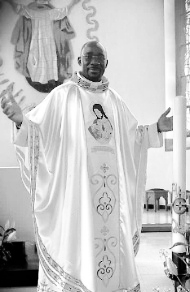
\includegraphics[scale=1.20]{../images/standing_daniel}
\end{wrapfigure}
Cette année nous porterons ensemble cette rentrée dans le cœur de chacun avec nos \textbf{jeunes pro}. Chacun à son rythme, selon ses possibilités et ses réalités mais avec un seul et même objectif : l’accomplissement de nos activités communautaires. Présentons également notre rentrée paroissiale au Christ. Et continuons notre chemin pour la mise en œuvre de notre projet paroissial autour de ce principal thème : \textbf{\og Avec notre jeunesse bâtissons une communauté plus dynamique, rayonnante et missionnaire\fg{}.}

	Que cette rentrée pastorale nous aide à prendre des résolutions nécessairement pour plonger à frais nouveaux dans la parole et être des disciples crédibles de l’évangile.


\begin{flushright}
Bonne rentrée pastorale à toutes et à tous !
\textit{Père  Daniel  ETTÉ}
\end{flushright}


\end{minipage}
%\end{center}
% -----
\end{document}
